\section{Discussion}
\label{sec:discussion}

The preference result and the defect result answer different questions, and they should not be averaged into one leaderboard.

On HPDv2 tattoo-subject pairs, human winners are the images our a-priori probes call worse to tattoo.
Dense shading, tight spacing and thin lines are attractive on a screen.
They are also the features a needle of width $w_n$ and a gap of width $g$ penalise.
A prompt-held-out fusion can predict the annotator, at \FusHpdProbespreregisteredAcc, only by flipping those penalties.
Using that fusion as a tattooability reward would optimise the opposite of the probe specification.
Using HPSv2.1 as a tattooability reward would do the same thing for a different reason: it agrees with the annotators (\HpdHpstwoAcc) on data it was trained on, and it has no millimetre scale.

Edge transition separates blur, detail loss and thickening from the clean image.
Mid-tone fraction separates haze and speckle.
Sub-needle fraction separates thinning.
The deprecated composite cancels some of those effects because thickening improves a width probe while hurting a gap probe.
Per-dimension reporting is the property the reward models do not have: HPSv2.1 detects most injected defects and does not name which geometric fact changed.

The Pick-a-Pic tattoo-subject slice is only \PapHpstwoN\ pairs.
Probe fusion there stays below one half (\FusPapProbespreregisteredAcc) and does not reproduce the HPDv2 sign flip in full.
Reward fusion is high (\FusPapRewardsAcc) with a positive PickScore coefficient, which is training leakage from Pick-a-Pic v1, not a new external test.
HPSv2.1 and ImageReward were not trained on that set; their Pick-a-Pic intervals are still wide.

ImageRewardDB does not rescue a positive probe--preference correlation.
The point estimates sit near chance, the prompt count is \NIrTsprompts, and ImageReward's own accuracy on that set is an in-distribution number with a wide interval.
A claim that ``rewards ignore tattooability'' is too broad: several rewards notice blur, haze and thinning in the injection study.
The supported claim is narrower.
Preference on the public tattoo-subject pairs we could score is not a tattooability label, and models trained to imitate that preference should not be described as if it were.

\begin{figure}[htbp]
  \centering
  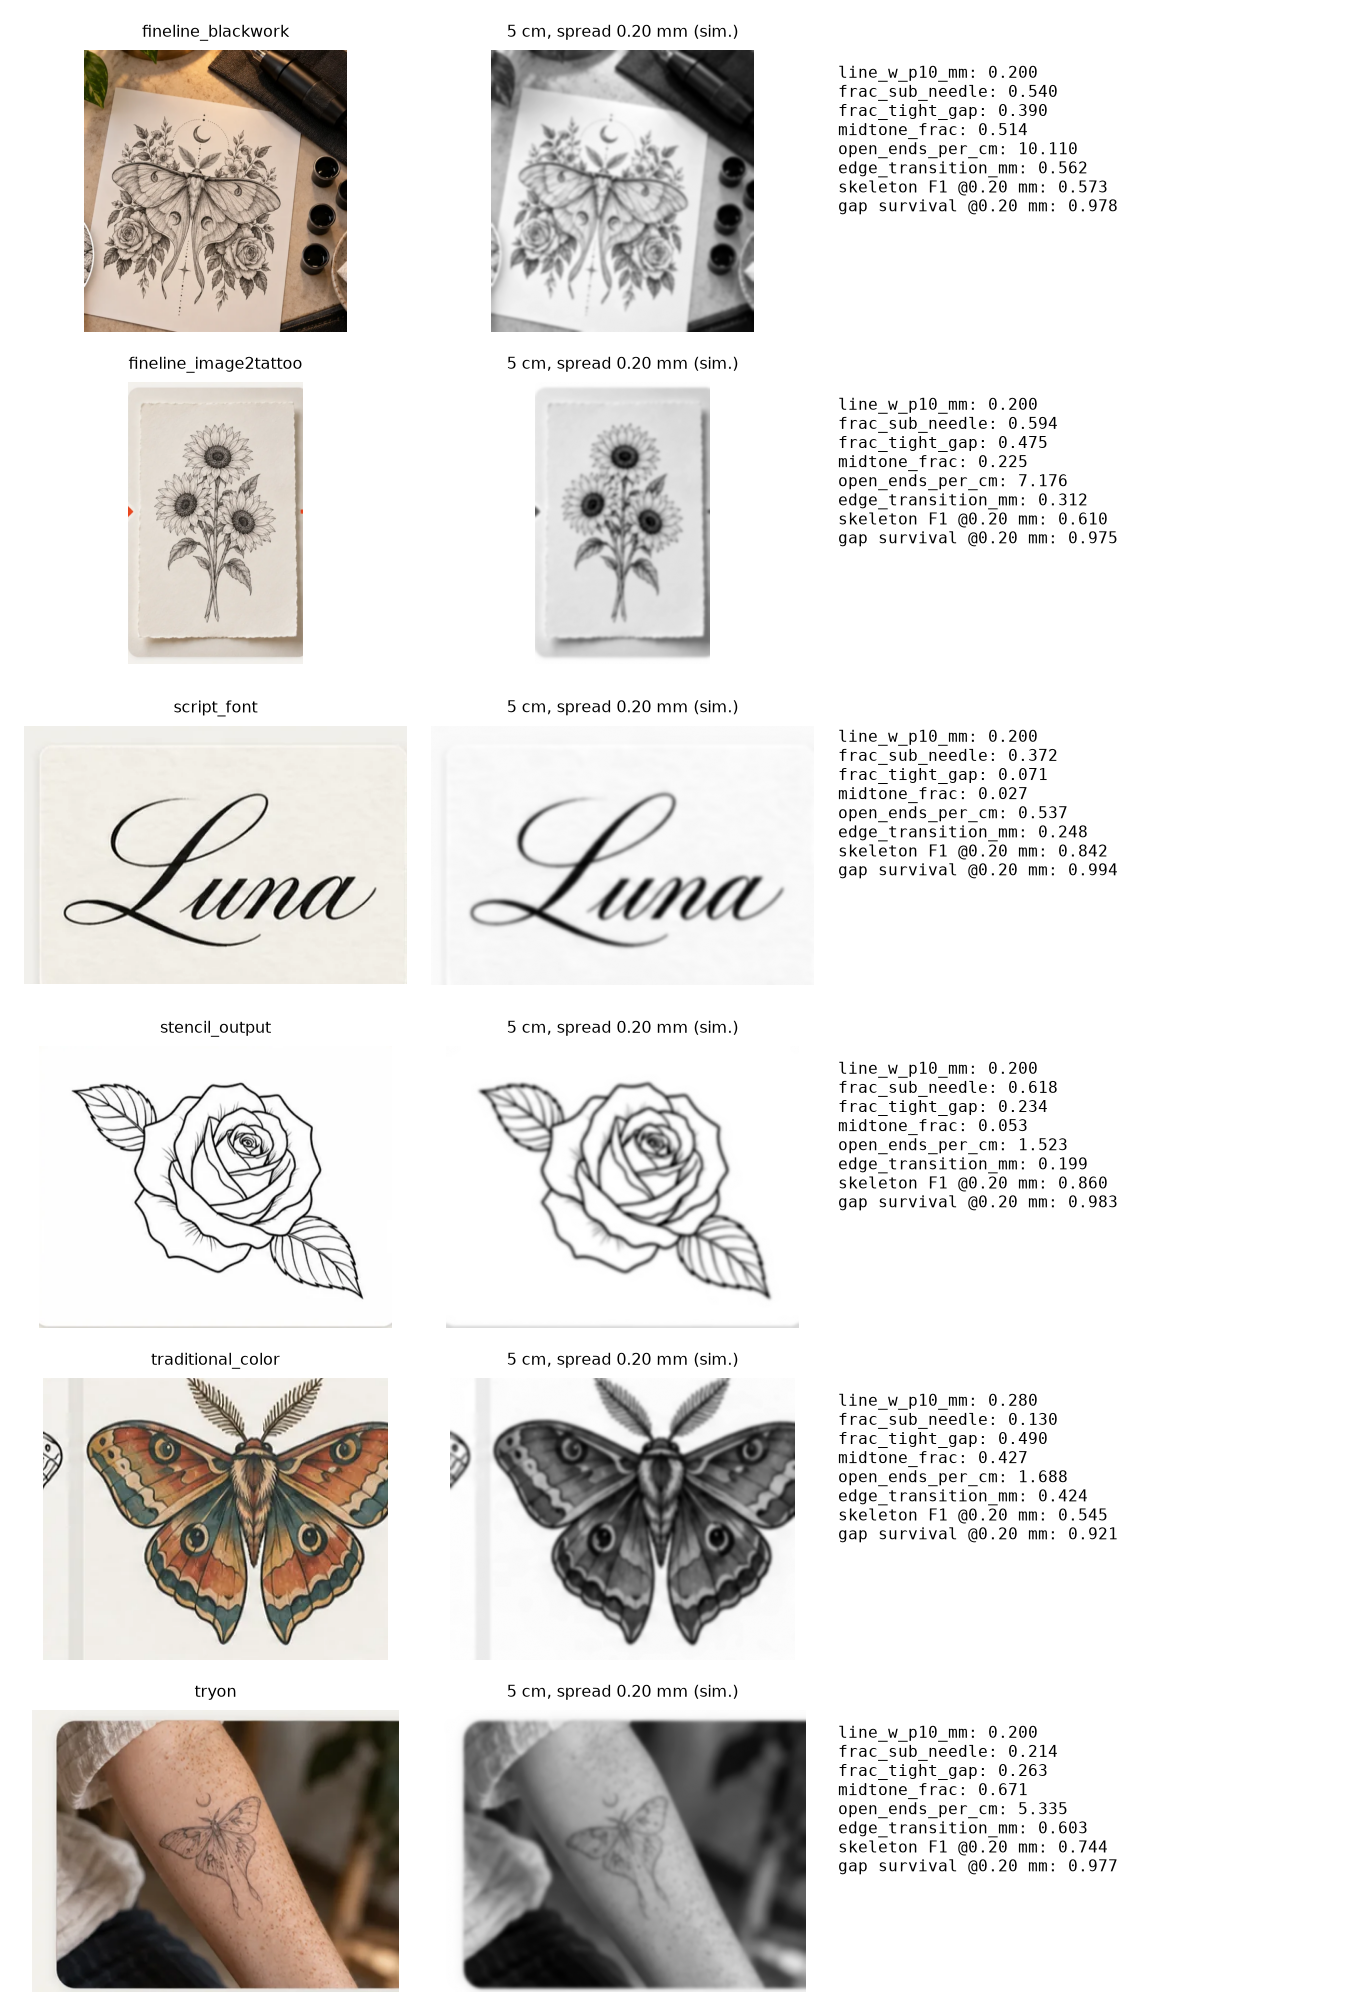
\includegraphics[width=0.92\linewidth]{figures/tatany_illustrative.png}
  \caption{The author operates tatany.app.
  The images are tatany.app product case images (marketing mock-ups cropped to one panel; provenance in supplementary notes).
  Probes at $s{=}5$\,cm and a simulated spread $\sigma{=}0.20$\,mm are shown for illustration only.
  tatany is not ranked, evaluated or compared with any other system.}
  \label{fig:tatany}
\end{figure}

A practical screen for AI tattoo generation can reject sub-needle line mass, tight gaps and soft transitions at the intended print size $s$.
Those gates disagree with current preference rewards on the HPDv2 pairs above.
That disagreement is a reason to keep the gates.
